\section{Homomorphic filtering: illumination and reflectance}

\textbf{Data.} \code{tunnel\_image.jpg} ($3644\times3000$, a phone photograph looking
along a dark tunnel towards a bright opening) is unevenly lit in exactly the way
the problem describes: deep shadow on the walls and floor and a bright, clipped
region at the far end. It was converted to luminance
$Y=0.299R+0.587G+0.114B$ in $[0,1]$ and box-averaged $4\times4$ to $911\times750$,
which keeps every structure of interest and makes a full parameter sweep quick.

\subsection{The multiplicative model}

Following the standard homomorphic model \cite{gonzalez}, the image is modelled as $I(x,y)=L(x,y)R(x,y)$, with illumination $L>0$ varying
slowly across the scene and reflectance $R\in(0,1]$ carrying edges and texture. A
linear filter cannot separate the two directly, because the Fourier transform of a
product is a convolution, $\mathcal{F}\{I\}=\mathcal{F}\{L\}\circledast\mathcal{F}\{R\}$:
every reflectance frequency is smeared by the illumination spectrum, so no
frequency band belongs to $L$ or to $R$ alone. Taking the logarithm first turns the
product into a sum,
\begin{equation}
z=\ln I=\ln L+\ln R,\qquad Z=\mathcal{F}\{z\}=\mathcal{F}\{\ln L\}+\mathcal{F}\{\ln R\},
\end{equation}
and the Fourier transform keeps that sum because it is linear. Since $\ln L$ is
smooth, its spectrum sits near the origin, while $\ln R$ has most of its energy at
higher frequencies. A filter $H$ with gain $\gamma_L<1$ near the origin and
$\gamma_H>1$ further out then acts on each part separately, and exponentiating
gives approximately
\begin{equation}
\hat I=\exp\big(\mathcal{F}^{-1}\{HZ\}\big)\approx L^{\gamma_L}R^{\gamma_H},
\end{equation}
which compresses the illumination range and stretches the reflectance contrast.

The log must come before the transform. The point of the log is to make the
spatial product additive, and it does so only when applied to the pixel values.
After the transform the product has already become a convolution, and the log of a
convolution is not a sum of anything useful. Filtering the log-magnitude spectrum
instead, $\log|G|=H\log|\mathcal{F}\{I\}|$, i.e.\ $|G|=|\mathcal{F}\{I\}|^{H}$ with the
original phase, is a fixed power law on spectral magnitudes. It is the same
operation for every pixel, so it cannot brighten dark regions more than lit ones,
and the phase is left paired with magnitudes it no longer belongs to.

A synthetic check makes this quantitative. With a Gaussian light $L$ from 0.03 to 1
and a block texture $R\in\{0.4,0.9\}$, the reflectance detail (mean $9\times9$ local
standard deviation) is 22.7 times larger in the lit region than in the dark one,
because the detail is scaled by $L$. Table~\ref{tab:logcheck} applies the same
$H$ ($D_0=20$, $\gamma_L=0.5$, $\gamma_H=1.5$) three ways.

\begin{table}[H]
\centering
\begin{tabular}{lrrr}
\toprule
Method & detail, lit & detail, dark & lit / dark\\
\midrule
input $I=LR$ & 0.2212 & 0.0097 & 22.69\\
filter $I$ directly & 0.3313 & 0.0146 & 22.73\\
filter $\log|\mathcal{F}\{I\}|$ & 3.7230 & 0.2250 & 16.55\\
filter $\log I$ (homomorphic) & 0.4468 & 0.0855 & 5.23\\
\bottomrule
\end{tabular}
\caption{Detail in lit ($L>0.9$) and dark ($L<0.06$) regions of the synthetic
scene (\code{log\_domain\_check.txt}).}
\label{tab:logcheck}
\end{table}

Filtering $I$ directly scales all detail by the same factor and leaves the ratio at
22.7. Filtering the log-magnitude spectrum changes it only to 16.6 and inflates the
values tenfold. The homomorphic filter brings the ratio to 5.23, close to the
$22.69^{\gamma_L}=4.76$ that $\hat I\approx L^{\gamma_L}R^{\gamma_H}$ predicts. It
is a little higher because the separation by frequency is not perfect: the block
texture has some low-frequency energy, which receives $\gamma_L$ rather than
$\gamma_H$.

\subsection{Implementation and tuning}

\code{homomorphic} in \code{src/problem\_3/homomorphic.py} computes
$z=\ln(I+1/255)$ (the offset keeps black pixels finite), mirror-pads $z$ to
$P=2\max(\text{rows},\text{cols})=1822$, multiplies the centred spectrum by
\begin{equation}
H(u,v)=(\gamma_H-\gamma_L)\big[1-e^{-cD^2(u,v)/D_0^2}\big]+\gamma_L,\qquad c=1,
\end{equation}
inverts, crops, and returns $e^{z'}-1/255$. Mirror padding replaces the zero
padding of Problem 2 here: zero is a very negative value in the log domain, and
zero padding would put a large artificial step at every border. To compare methods
on equal terms, every output, the input included, is mapped to $[0,1]$ by its own
0.1 and 99.9 percentiles.

The measurements use two regions defined from the input: the shadow is the darkest
25\,\% of the $31\times31$ smoothed luminance (170813 pixels: floor, lower walls,
corners), and the bright region is the top 1\,\% (6833 pixels: the opening).
Shadow and bright contrast are the mean $15\times15$ local standard deviation in
those regions, ``bright sat.'' is the share of bright pixels at or above 0.98,
``levels'' counts distinct 8-bit output values in the shadow, and ``reversal''
measures halos. It is the share of the strongest 25\,\% of input gradients, both
images smoothed with a $15\times15$ box, whose direction the output reverses. A
global monotone tone curve cannot reverse a smoothed gradient, so this is close to
zero for histogram equalisation; a halo is precisely a band beside a large edge
where the output slopes the wrong way.

\begin{table}[H]
\centering
\small
\begin{tabular}{rrrrrrrrrr}
\toprule
$D_0$ & $\gamma_L$ & $\gamma_H$ & shadow contr. & bright contr. & bright sat. & blown out & levels & shadow mean & reversal\\
\midrule
\multicolumn{3}{l}{input} & 0.0015 & 0.0033 & 1.000 & 0.0116 & 7 & 0.0110 & 0.0000\\
\midrule
10 & 0.25 & 1.25 & 0.0142 & 0.0157 & 0.076 & 0.0030 & 87 & 0.2347 & 0.0872\\
10 & 0.25 & 2.00 & 0.0157 & 0.0237 & 0.012 & 0.0021 & 87 & 0.2175 & 0.1094\\
10 & 0.50 & 1.50 & 0.0074 & 0.0149 & 0.101 & 0.0030 & 41 & 0.1010 & 0.0495\\
10 & 0.75 & 1.25 & 0.0034 & 0.0085 & 0.313 & 0.0050 & 15 & 0.0306 & 0.0083\\
40 & 0.25 & 1.25 & 0.0186 & 0.0082 & 0.000 & 0.0024 & 102 & 0.3087 & 0.0966\\
40 & 0.25 & 2.00 & 0.0224 & 0.0111 & 0.000 & 0.0014 & 110 & 0.3185 & 0.1323\\
40 & 0.50 & 1.50 & 0.0096 & 0.0076 & 0.071 & 0.0035 & 47 & 0.1305 & 0.0531\\
40 & 0.50 & 2.00 & 0.0117 & 0.0106 & 0.001 & 0.0024 & 55 & 0.1536 & 0.0773\\
40 & 0.75 & 1.25 & 0.0039 & 0.0047 & 0.475 & 0.0070 & 16 & 0.0342 & 0.0085\\
160 & 0.25 & 1.25 & 0.0195 & 0.0032 & 0.006 & 0.0025 & 85 & 0.2420 & 0.0226\\
160 & 0.25 & 2.00 & 0.0261 & 0.0045 & 0.000 & 0.0017 & 111 & 0.3109 & 0.0470\\
160 & 0.50 & 1.50 & 0.0094 & 0.0032 & 0.991 & 0.0127 & 37 & 0.0915 & 0.0058\\
\textbf{160} & \textbf{0.50} & \textbf{2.00} & \textbf{0.0117} & \textbf{0.0040} & \textbf{0.012} & \textbf{0.0023} & \textbf{46} & \textbf{0.1205} & \textbf{0.0137}\\
160 & 0.75 & 1.25 & 0.0037 & 0.0030 & 1.000 & 0.0121 & 13 & 0.0233 & 0.0002\\
160 & 0.75 & 2.00 & 0.0054 & 0.0039 & 0.989 & 0.0123 & 20 & 0.0458 & 0.0035\\
\bottomrule
\end{tabular}
\caption{Selected rows of the 27-setting sweep (all rows in
\code{sweep\_metrics.txt}). Bold: the setting chosen as good.}
\label{tab:sweep}
\end{table}

\begin{figure}[H]
\centering
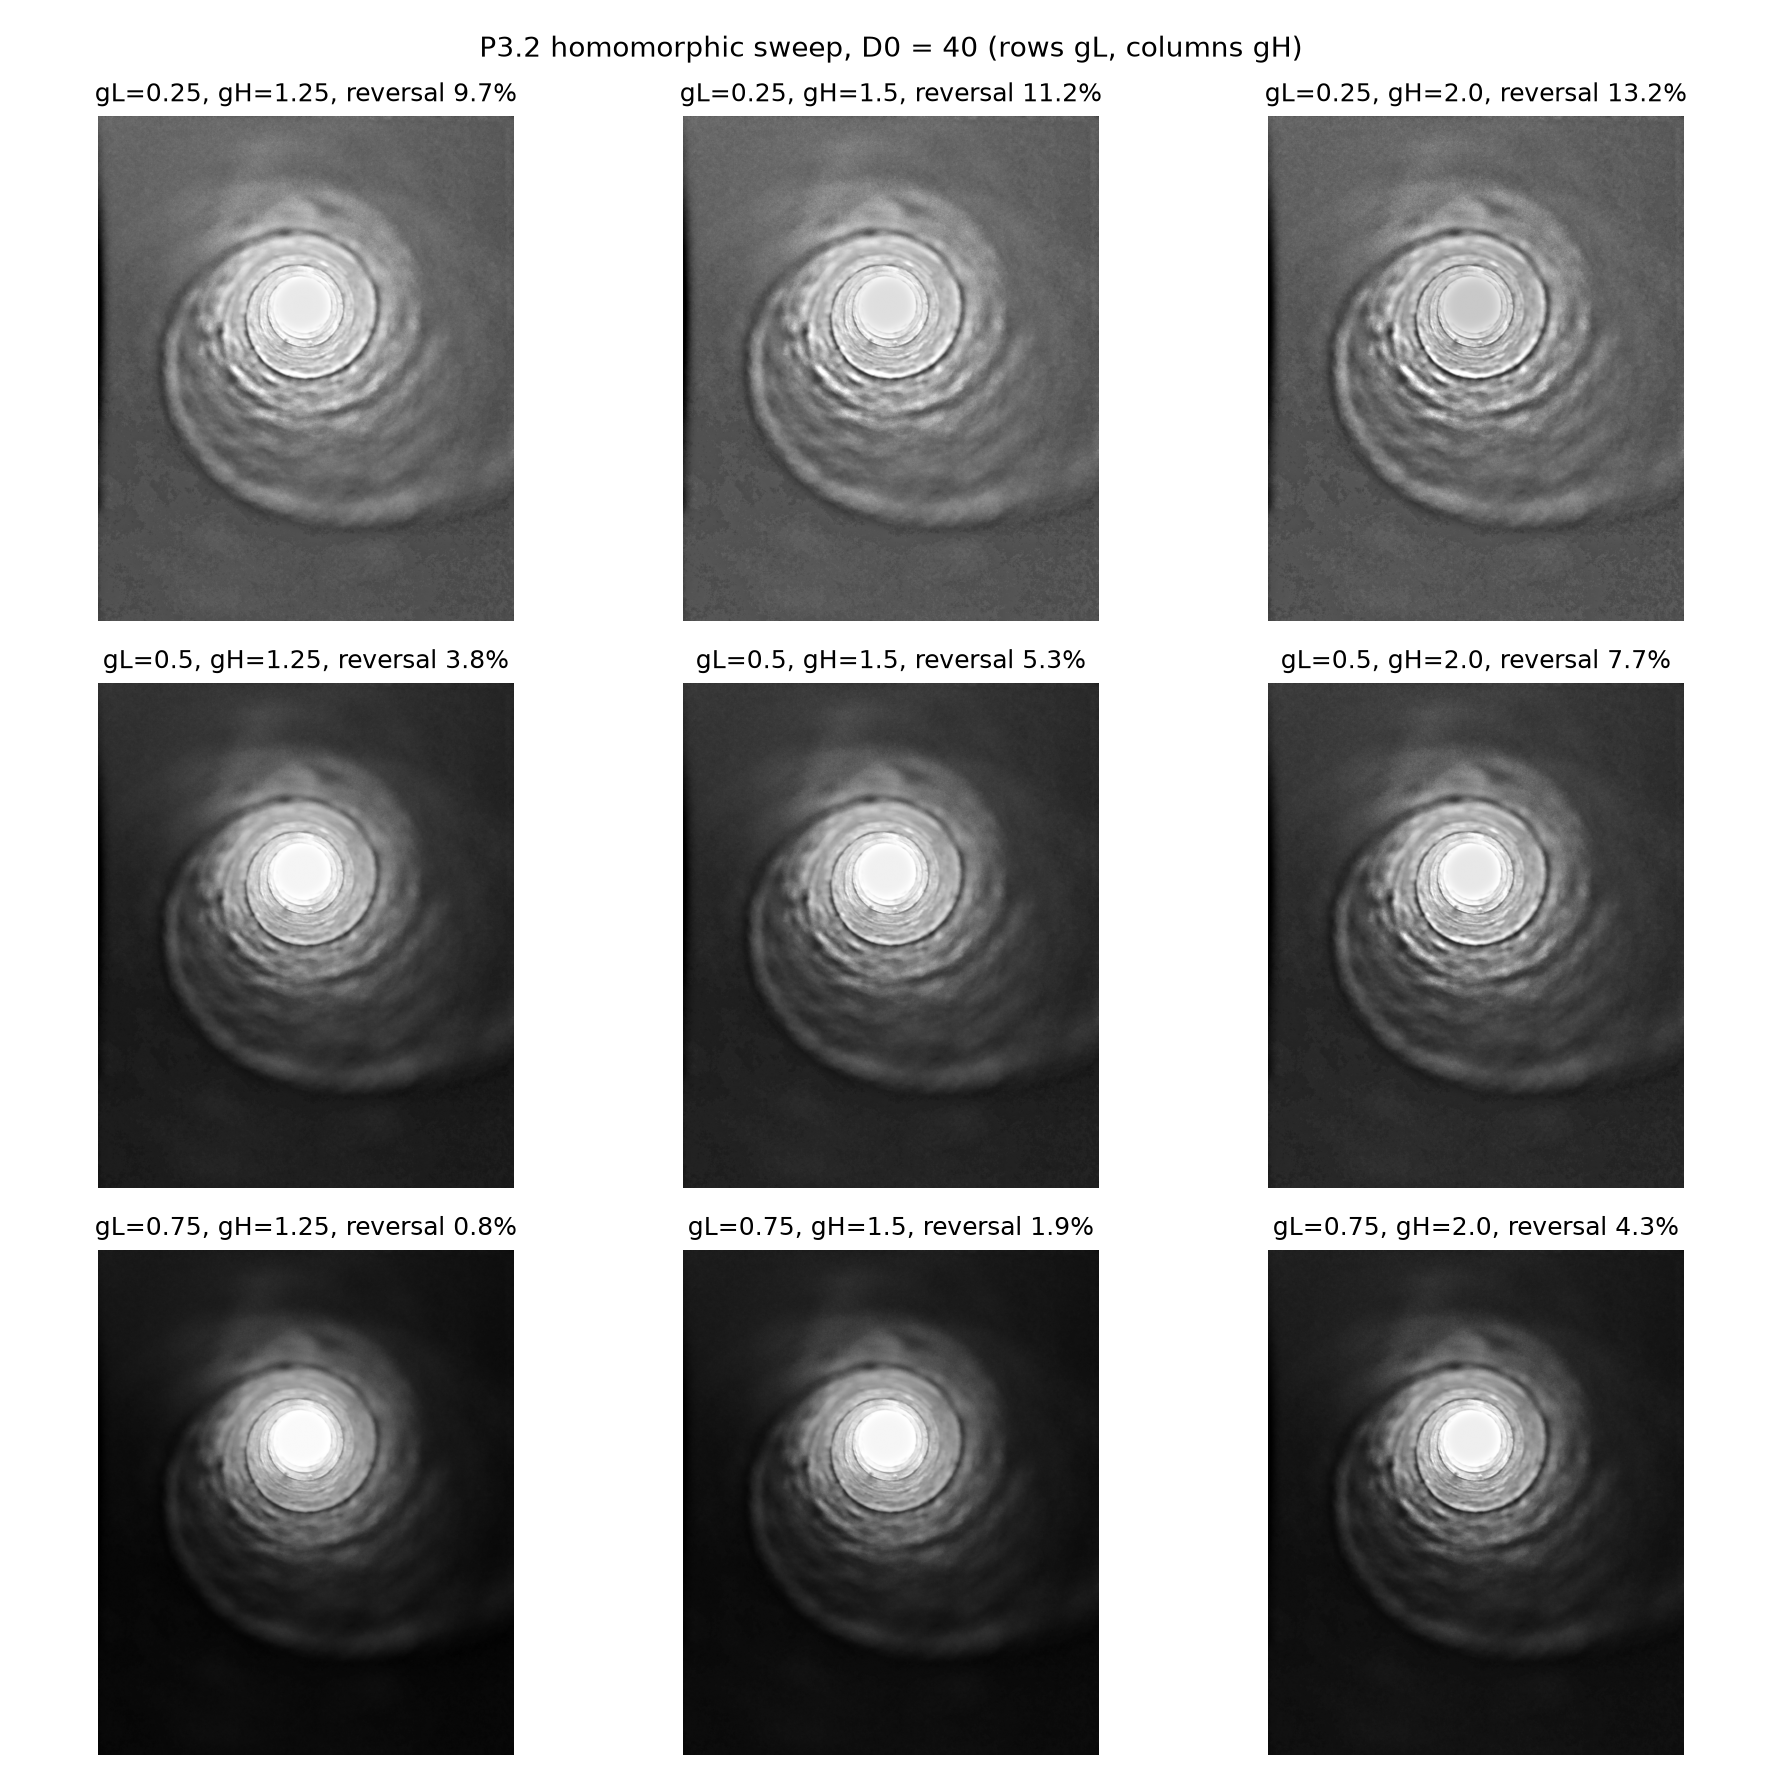
\includegraphics[width=0.49\linewidth]{problem_3/sweep_grid_d0_40.png}
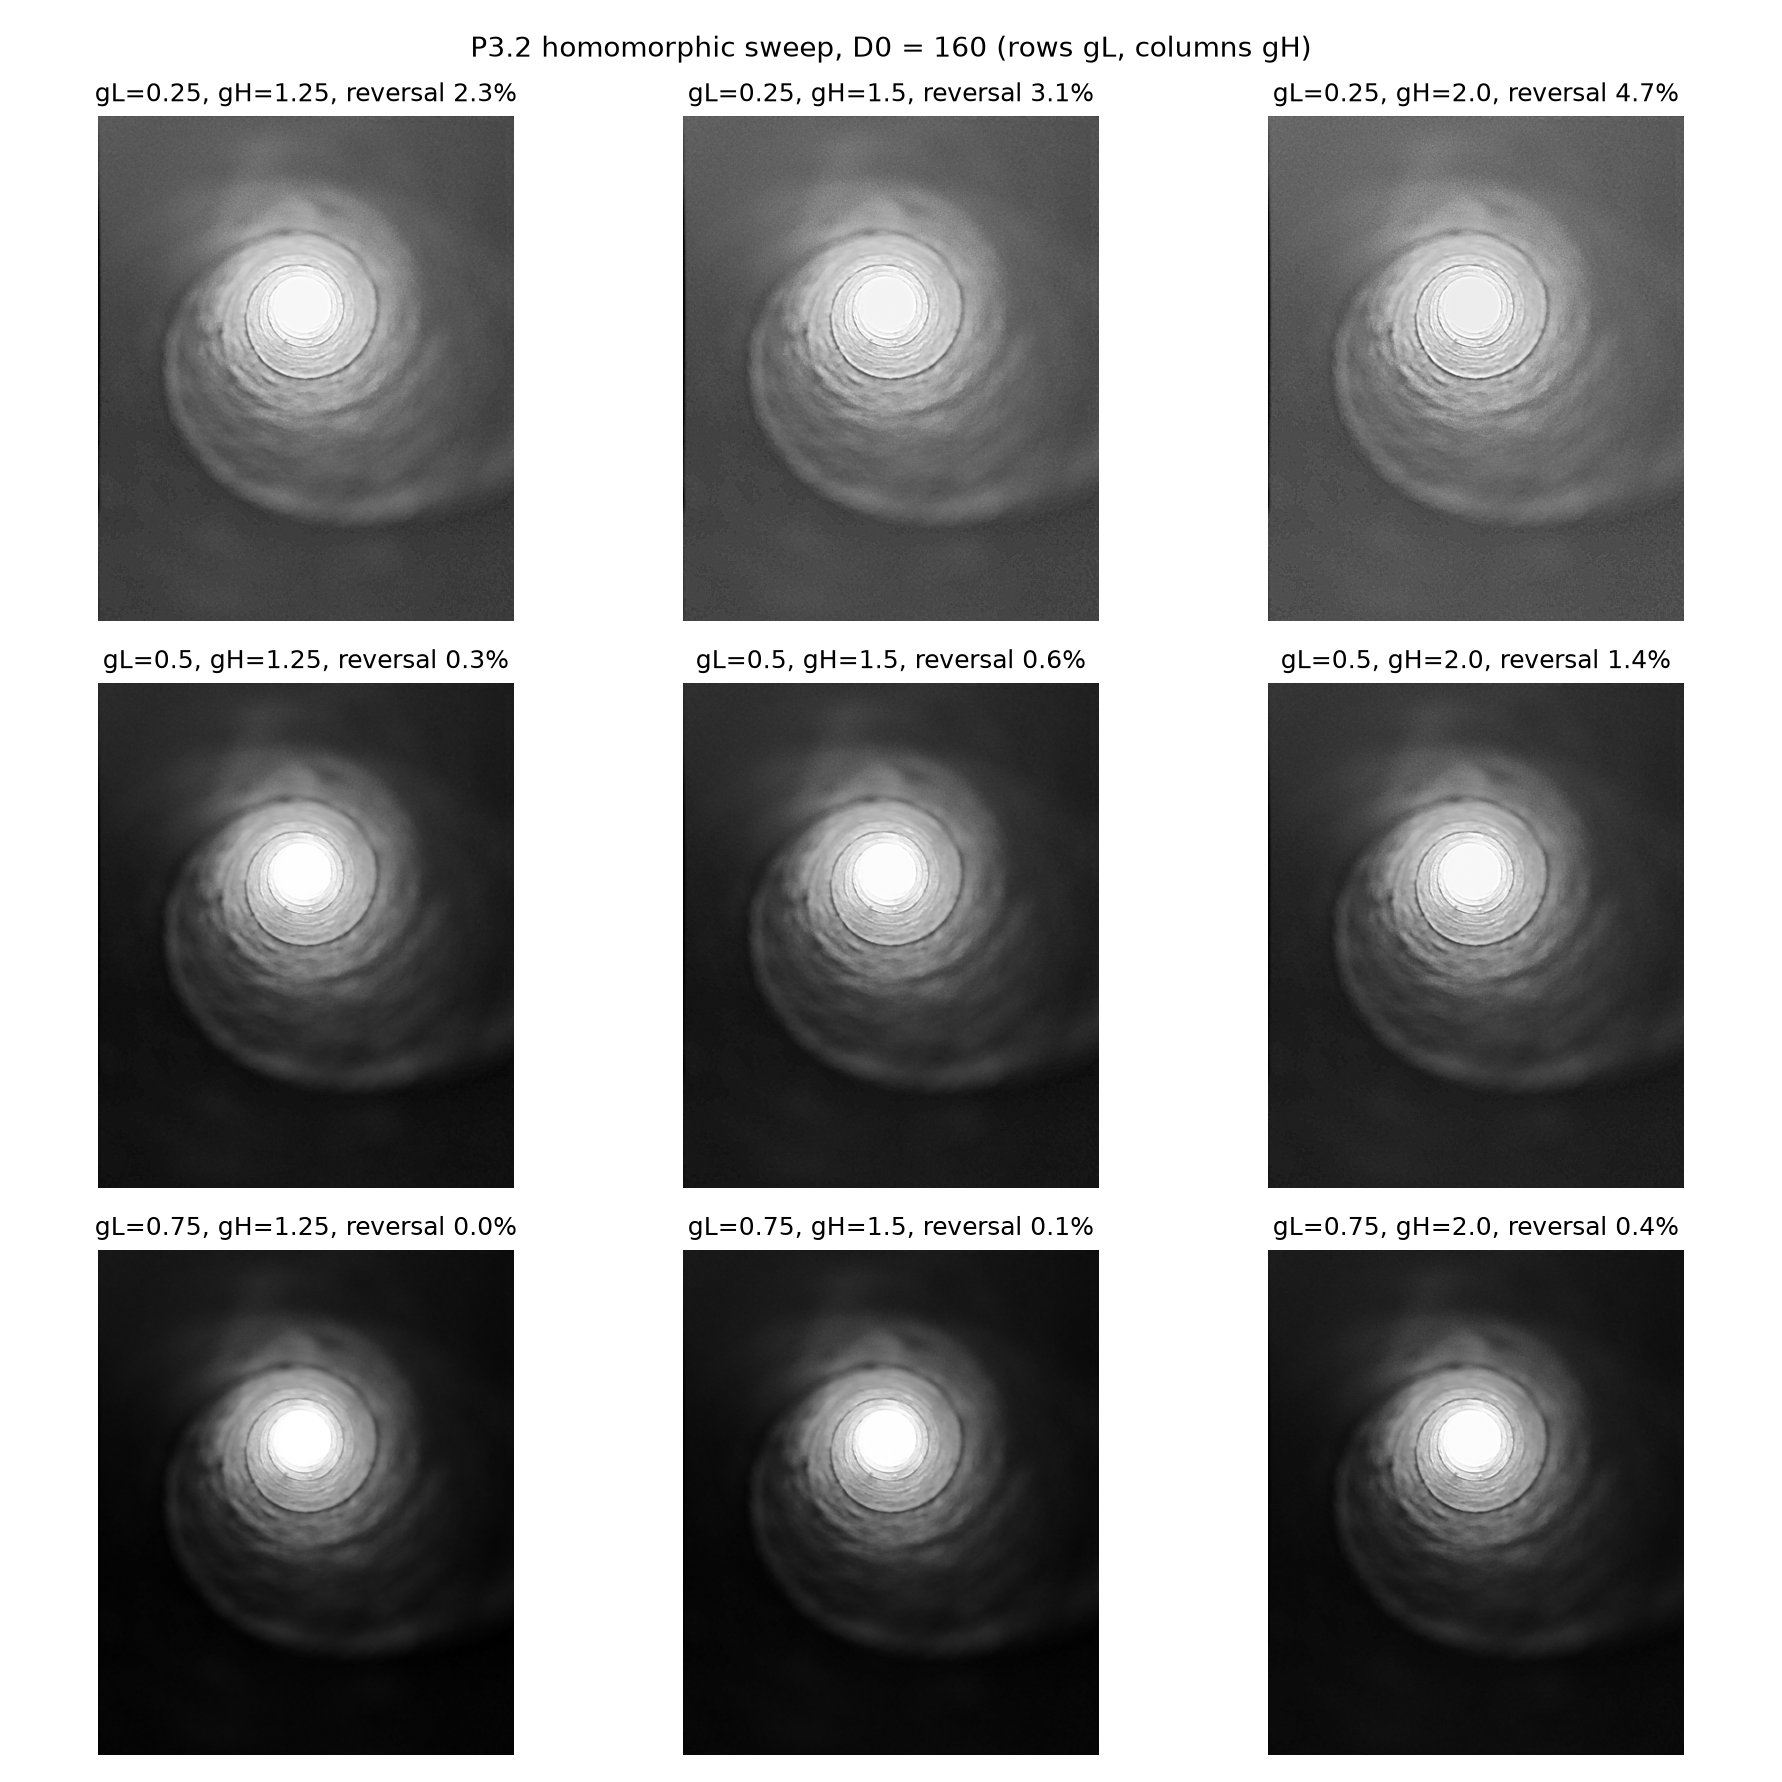
\includegraphics[width=0.49\linewidth]{problem_3/sweep_grid_d0_160.png}
\caption{Sweep grids for $D_0=40$ (left) and $D_0=160$ (right): rows
$\gamma_L=0.25,0.5,0.75$, columns $\gamma_H=1.25,1.5,2$. The $D_0=10$ grid is in
\code{sweep\_grid\_d0\_10.png}.}
\label{fig:sweep}
\end{figure}

The parameters act as the model says. $\gamma_L$ sets how much the illumination is
flattened: going from 0.75 to 0.25 lifts the mean shadow level from 0.02--0.07 to
0.22--0.32 at every $D_0$. $\gamma_H$ sets the detail gain, and the contrast in both
regions rises with it. $D_0$ sets the scale that counts as illumination. The
low-pass part $e^{-D^2/D_0^2}$ is a Gaussian with spatial standard deviation
$\sigma=\sqrt2\,P/(2\pi D_0)$, i.e.\ 41, 10 and 2.6 pixels for $D_0=10$, 40 and 160.

\textbf{Halos} appear where strong flattening ($\gamma_L=0.25$) meets strong
emphasis ($\gamma_H=2$), and they are worst at $D_0=40$: reversal 13.2\,\% at
$(40,0.25,2)$, against 10.9\,\% at $D_0=10$ and 4.7\,\% at $D_0=160$. The filter
behaves like unsharp masking in the log domain, and every large edge gets an over-
and undershoot band about $\sigma$ wide. At $D_0=40$ the bands are about 10 pixels
wide, the same scale as the rings of the tunnel and the rim of the opening, so they
read as bright and dark contours; Fig.~\ref{fig:sweep} (left, top row) shows
them around the light. At $D_0=160$ they are too thin to be visible as halos, and at
$D_0=10$ they are broad and gentle.

\textbf{Good settings.} No setting stays below 1\,\% reversal without leaving the
light saturated, so the rule was set at reversal $\le2\,\%$ and bright saturation
$\le10\,\%$, then the largest shadow contrast. Like the rule in 2.3b, these limits
were chosen after seeing the table. The rule selects $(D_0,\gamma_L,\gamma_H)=(160,0.5,2)$:
shadow contrast 7.8 times the input's, mean shadow level up from 0.0110 to 0.1205,
1.2\,\% of the light saturated, and 1.4\,\% gradient reversal.

One caution about the bright region: 98.3\,\% of its full-resolution pixels have at
least one channel at 255, so the light is clipped in the JPEG itself. A setting that
lowers ``bright sat.'' maps that flat clipped area below white; it does not recover
detail that was never recorded. Indeed, at $D_0=160$ with $\gamma_H\le1.5$ the light
stays saturated, while $\gamma_H=2$ creates small overshoots at its rim that take
the top percentile and push the flat interior below 0.98.

\subsection{Comparison with histogram equalisation}

Global histogram equalisation uses the Assignment 1 implementation,
$T(v)=\operatorname{round}(255F(v))$ on the 8-bit luminance, with $F$ the inclusive
cumulative histogram.

\begin{table}[H]
\centering
\small
\begin{tabular}{lrrrrrrr}
\toprule
Method & shadow contr. & bright contr. & bright sat. & blown out & levels & shadow mean & reversal\\
\midrule
input & 0.0015 & 0.0033 & 1.000 & 0.0116 & 7 & 0.0110 & 0.0000\\
histogram equalisation & 0.0321 & 0.0015 & 1.000 & 0.0218 & 7 & 0.1670 & 0.0005\\
homomorphic $(160,0.5,2)$, good & 0.0117 & 0.0040 & 0.012 & 0.0023 & 46 & 0.1205 & 0.0137\\
homomorphic $(40,0.25,2)$, halo & 0.0224 & 0.0111 & 0.000 & 0.0014 & 110 & 0.3185 & 0.1323\\
\bottomrule
\end{tabular}
\caption{Local contrast and side effects (\code{local\_contrast.txt}).}
\label{tab:he}
\end{table}

\begin{figure}[H]
\centering
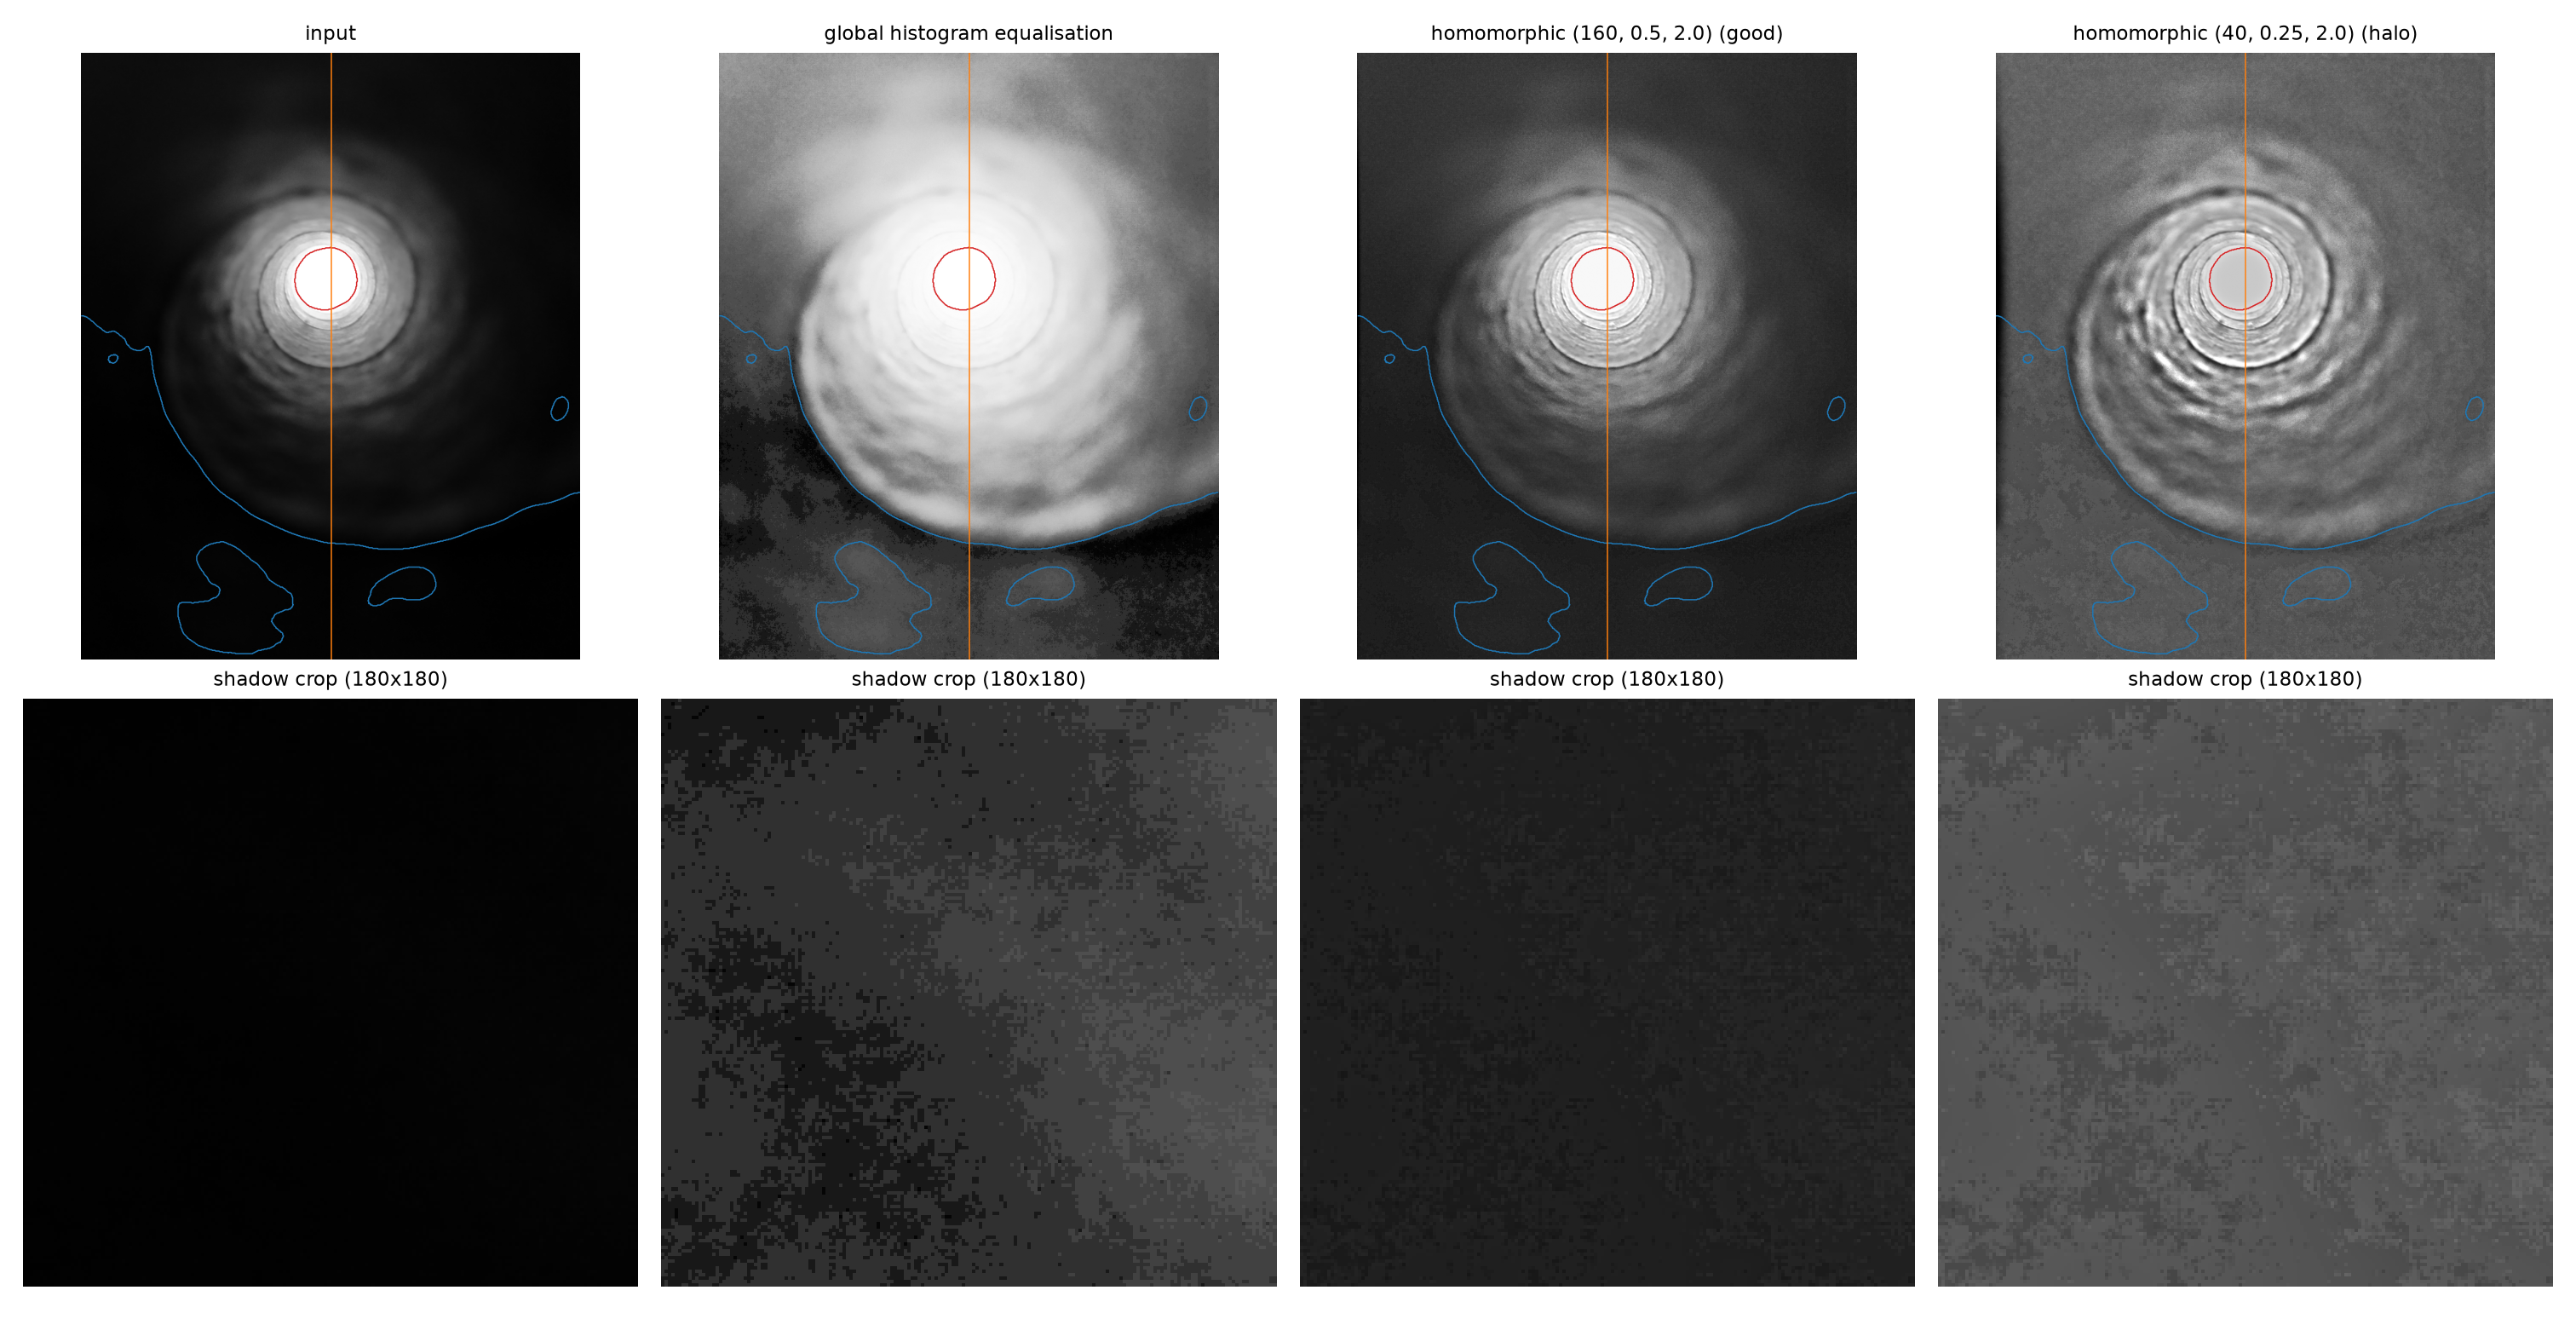
\includegraphics[width=\linewidth]{problem_3/homomorphic_comparison.png}
\caption{Input, equalisation and two homomorphic settings, with the shadow region
(blue) and bright region (red) outlined and a $180\times180$ shadow crop below.}
\label{fig:homo}
\end{figure}

\begin{figure}[H]
\centering
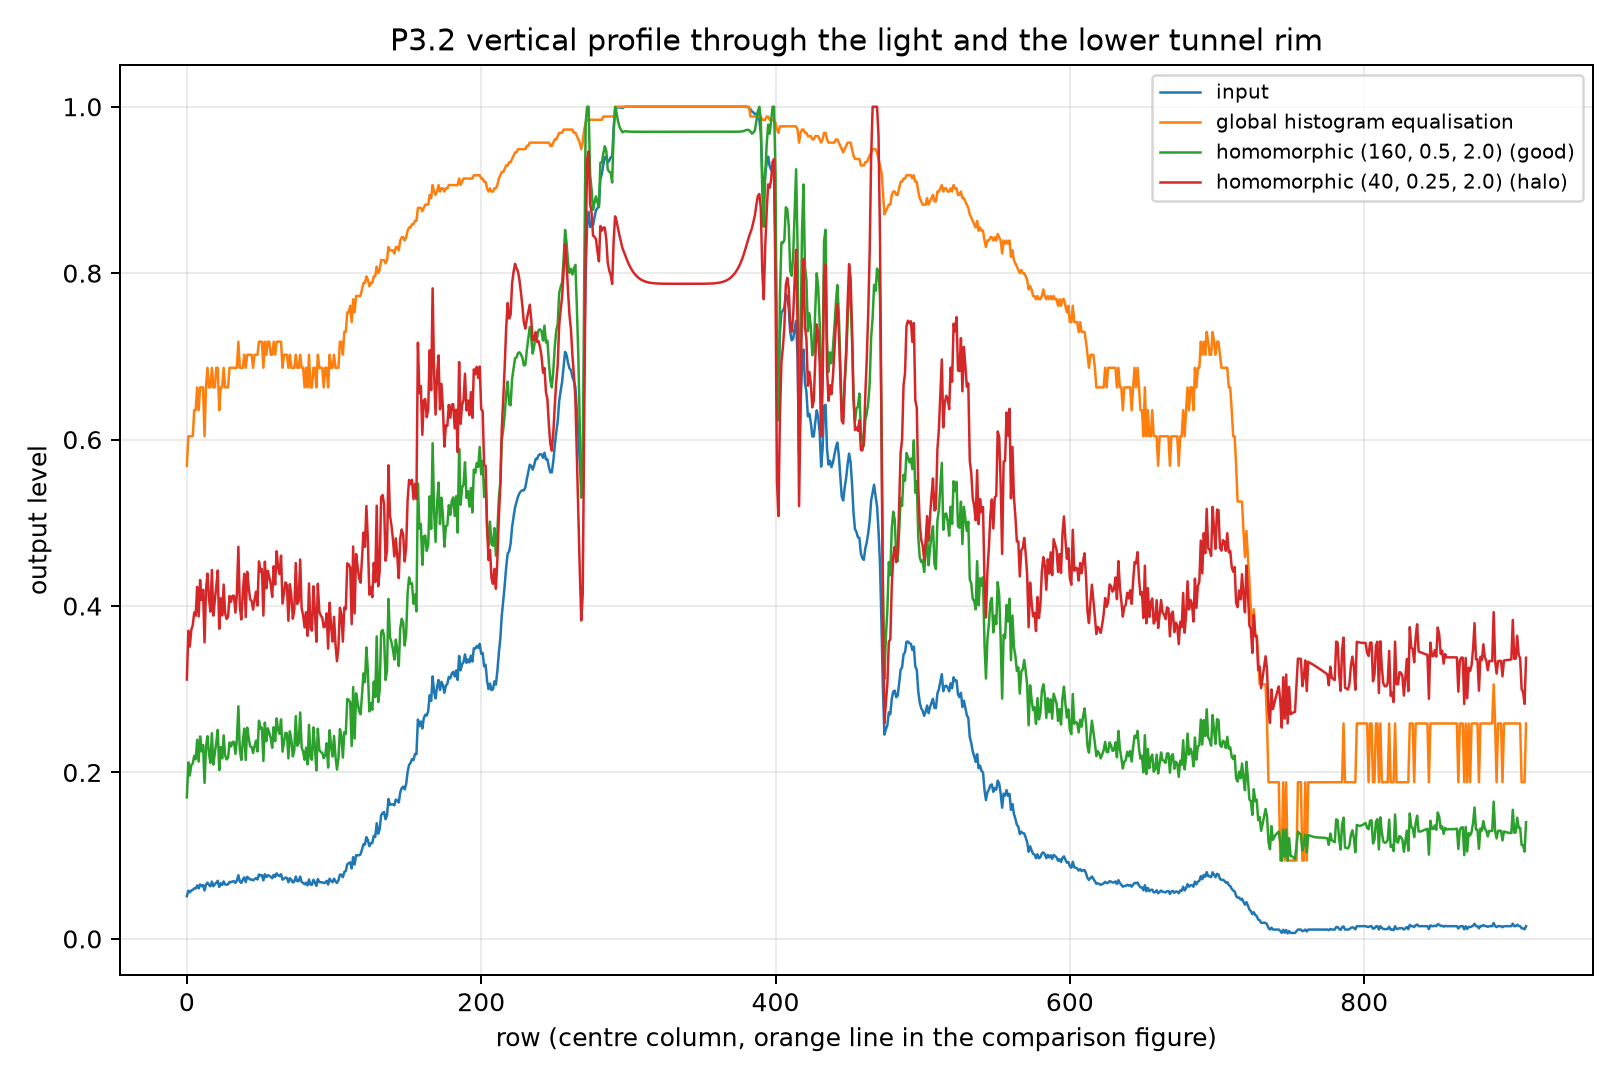
\includegraphics[width=0.75\linewidth]{problem_3/profiles.png}
\caption{Vertical profile through the centre column (orange line in
Fig.~\ref{fig:homo}).}
\label{fig:homo-profile}
\end{figure}

By raw local standard deviation, equalisation wins in the shadow (0.0321 against
0.0117), but that number is not recovered detail. The shadow of the input occupies
only seven distinct 8-bit values, and a look-up table cannot create new ones, so
equalisation spreads those seven values far apart. Its shadow ``contrast'' is the
quantisation steps and sensor noise made visible as blotchy posterisation
(Fig.~\ref{fig:homo}, shadow crop; the staircase in Fig.~\ref{fig:homo-profile}).
It also pushes most of the lit tunnel wall towards white (blown-out share up from
1.16\,\% to 2.18\,\%), and the light remains fully saturated. Equalisation allocates
output range by pixel counts over the whole image and has no notion of what is
illumination and what is reflectance.

The good homomorphic setting lifts the shadow by a factor of about 11 in mean level
and 7.8 in local contrast, renders it with 46 distinct levels instead of 7 (each
output pixel depends on its neighbourhood, so the filter interpolates between the
quantised input values), keeps the lit walls away from white (0.23\,\% blown out)
and has no visible halos. It therefore recovers shadow detail better without
blowing out the bright region. The reason is the one in 3.1: it compresses $L$ and
keeps $R$, so contrast in the dark is raised by the same factor as the
illumination is lowered. Two limits remain. Detail that the 8-bit file never
recorded cannot be recovered by either method, and pushing for more shadow
contrast with $\gamma_L=0.25$ produces the halos of the $(40,0.25,2)$ setting, whose
profile maps the clipped light to a flat plateau at 0.79 with spikes to 1.0 at its
rim (Fig.~\ref{fig:homo-profile}).

\paragraph{Conclusion.} The log turns $I=LR$ into a sum that a linear filter can
split by frequency, which the synthetic check confirms (detail ratio 22.7 reduced
to 5.2, with 4.8 predicted). On the tunnel image, homomorphic filtering lifts the
shadows without saturating the walls. Strong flattening and emphasis at the scale
of the scene's large structures produces halos, which the gradient-reversal measure
detects.
